\documentclass[ex]{exercise}

\deadline{31.10.2023}

\begin{document}

\section{Listingsche Strahlenkonstruktion an Hohl- und Wölbspiegeln}
\hfill(siehe hinten)\hspace*{\fill}

\section{Brechungsindex einer Linse}
Ausgangspunkt sei die Linsenmachergleichung. Da es sich um eine dünne Linse handelt
ist \(d=0\), au{\ss}erdem ist \(r_2=\infty\); dies entspricht der ebenen Seite der Linse.
\begin{align*}
    \frac {n_0}f &= (n_L - n_0)\hug{\frac 1{r_1} + \frac 1{r_2}}
    + \frac{(n_L - n_0)^2}{n_L}\frac{d}{r_1r_2}\\
    \frac {n_0}f &= (n_L - n_0)\frac 1{r_1}\\
    n_L &= n_0\hug{\frac {r_1}f + 1}\\
    &\approx \frac{12 \u{cm}}{30 \u{cm}} + 1\\
    &\approx 1.4
\end{align*}

\section{Brennweite einer Linse bestimmen}
Ausgangspunkt sei die Linsenmachergleichung, da es sich um eine dünne Linse handelt.
\begin{align*}
    \frac{1}{f} &= \frac{1}{b} + \frac{1}{g} \\  
    \frac{1}{f} &= \frac{1}{L-g} + \frac{1}{g} \\  
    \frac{1}{f} &= \frac{L}{g(L-g)} \\   
    0 &= g^2 - gL + Lf \\  
    g &= \frac{L}{2} \pm \sqrt{\frac{L^2}{4} - Lf}\\
\end{align*}

\begin{enumerate}
    \item Fall \(\frac{L}{4} - f = 0\):
    In diesem Fall ist steht die Linse genau in der Mitte, und es gibt keine zwei 
    verschiedenen Positionen die eine scharfes Bild ergeben, somit entfällt dieser Fall im Rahmen 
    der Aufgabe.\\
    
    \item Fall \(\frac{L}{4} - f < 0\):
    In diesem Fall wird die Wurzel imaginär, physikalisch gesehen gibt es nun keine
    Position der Linse die ein scharfes Bild produziert. Auch dieser Fall entfällt.

    \item Fall \(\frac{L}{4} - f > 0\):
    In diesem Fall gibt es zwei verschiedene Positionen in denen die Linse ein scharfes Bild
    produziert, einmal vergrö{\ss}ert, einmal verkleinert.
    Die Distanz zwischen den beiden Positionen ist gegeben durch \(e = 2\sqrt{\frac{L^2}{4} - Lf}\).
    Im Folgenem wird dieser Fall angenommen.
\end{enumerate}

\begin{align*}
    g &= \frac{L}{2} \pm \frac e2\\
    \frac{1}{f} &= \frac{1}{L-g} + \frac{1}{g} \\
    &= \frac{1}{L-\frac{L}{2} \mp \frac e2} + \frac{1}{\frac{L}{2} \pm \frac e2} \\
    &= \frac{\frac L2  \pm \frac e2 + \frac L2 \mp \frac e2}{\frac{L^2}{4} - \frac {e^2}{4}} \\
    f &= \frac{L^2 - e^2}{4L}
\end{align*}

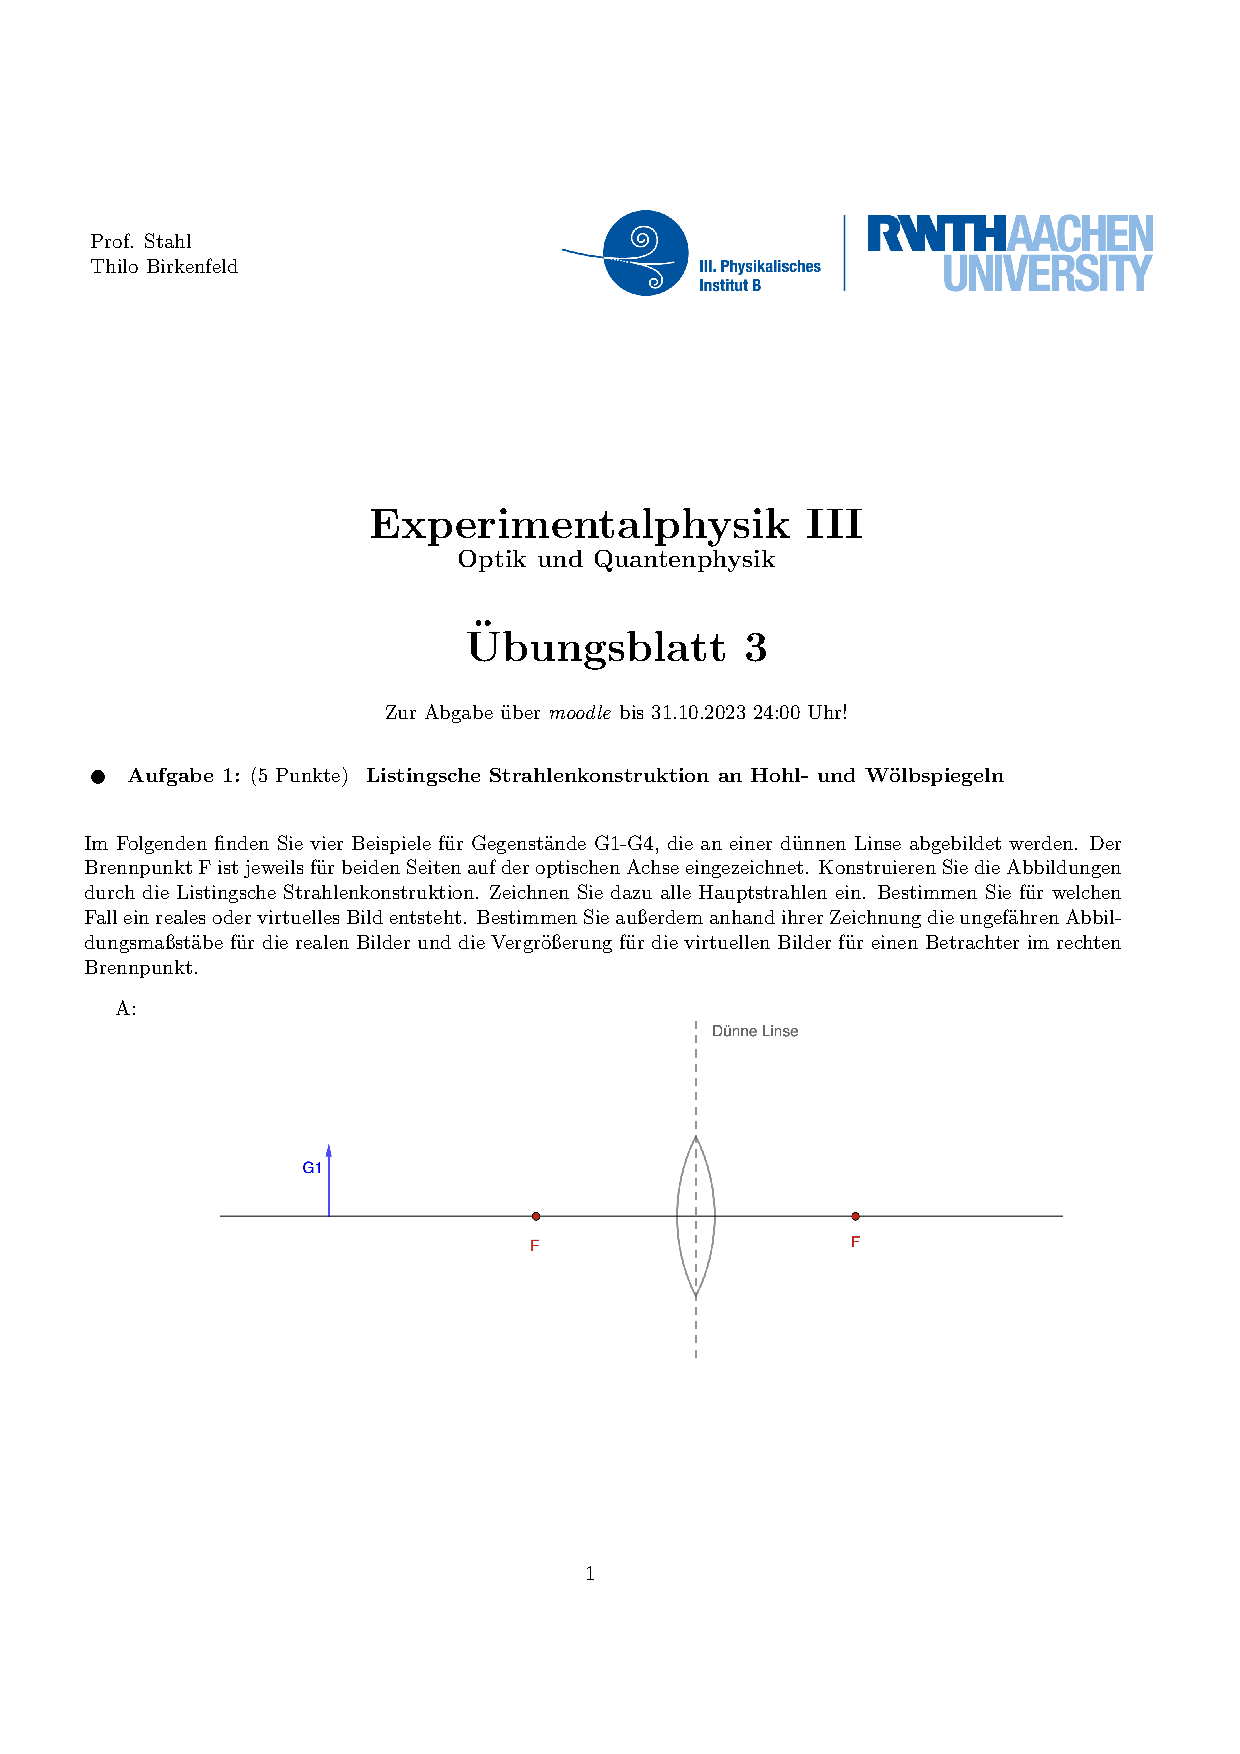
\includepdf[pages=1-2]{blatt3.pdf}

\end{document}